\documentclass{amsart}
\usepackage[margin=3cm]{geometry}


\usepackage{amssymb}

\usepackage[mathcal]{euscript}
\usepackage{relsize}

\usepackage{tikz}
\usepackage{tikz-cd}
% for a goodlooking table of contents
\let\oldtocsection=\tocsection 
\let\oldtocsubsection=\tocsubsection 
\renewcommand{\tocsection}[2]{\hspace{0mm}\oldtocsection{#1}{#2}}
\renewcommand{\tocsubsection}[2]{\hspace{1em}\oldtocsubsection{#1}{#2}}


\usepackage{hyperref}
\hypersetup{
    colorlinks,
    citecolor=black,
    filecolor=black,
    linkcolor=black,
    urlcolor=black
}


\usepackage{comment}
%

%symbols
\DeclareFontFamily{OT1}{pzc}{}
\DeclareFontShape{OT1}{pzc}{m}{it}{<-> s * [1.100] pzcmi7t}{}
\DeclareMathAlphabet{\mathpzc}{OT1}{pzc}{m}{it}


%for bold headers
   \usepackage{etoolbox}
    \patchcmd{\section}{\scshape}{\large\bfseries}{}{}
    \makeatletter
    \renewcommand{\@secnumfont}{\bfseries}
    \makeatother


\usepackage{quiver}
%tikz with options
\usepackage{tikz-cd}
% \tikzcdset{arrow style=math font}
% \tikzcdset{scale cd/.style={every label/.append style={scale=#1},
%     cells={nodes={scale=#1}}}}


%bibliography
%%%%%%%%%%%%%%%%%%%%%%%%%%%%%%%%%%%%%%%
% \usepackage{biblatex}
\bibliographystyle{plain}
\usepackage{booktabs}
\bibliography{references}
%---------------------------------






%-------------------




\numberwithin{equation}{section}
\newtheorem{theorem}{Theorem}[section]
\newtheorem*{theorem*}{Theorem}
\newtheorem{corollary}[theorem]{Corollary}
\newtheorem{lemma}[theorem]{Lemma}
\newtheorem{proposition}[theorem]{Proposition}
\theoremstyle{definition}
\newtheorem{question}{Question}
\newtheorem{problem}{Problem}
\newtheorem{definition}[theorem]{Definition}
\newtheorem*{definition*}{Definition}
\newtheorem{remark}[theorem]{Remark}
\newtheorem{example}[theorem]{Example}


\def\Grp{\mathsf{Grp}}
\def\Cov{\mathsf{Cov}}
\def\Subgroup{\mathsf{Subgroup\;}}
\def\Arr{\mathsf{Arr}}
\def\Obj{\mathsf{Obj}}
\def\Set{\mathsf{Set}}
\def\CC{\mathsf{C}}
\def\Cat{\mathsf{Cat}}
\def\Gpd{\mathsf{Gpd}}
\def\Set{\mathsf{Set}}
\def\Hom{\mathsf{Hom}}
\def\ZZ{\mathbb{Z}}
\def\RR{\mathbb{R}}
\def\id{\mathsf{id}}
\def\Id{\mathsf{Id}}

\newcommand{\F}{\mathcal{F}}
\newcommand{\cc}{\mathcal{C}}
\newcommand{\ww}{\mathcal{W}}
\newcommand{\qq}{\mathcal{Q}}
\newcommand{\ee}{\mathcal{E}}
\newcommand{\ii}{\mathcal{I}}
\newcommand{\bb}{\mathcal{B}}
\newcommand{\Eps}{\mathcal{E}}
\newcommand{\dd}{\mathcal{D}}
\newcommand{\Aut}{\mathrm{Aut}}
\newcommand{\colim}{\mathrm{colim}}
\newcommand{\dom}{\mathrm{dom}}
\newcommand{\cod}{\mathrm{cod}}

\newcommand{\Tau}{\mathcal{T}}
\newcommand{\Crossed}{\textsf{Crossed}}
% % \def\Crossed{\textsf{Crossed}}
% \DeclareMathOperator{\Crossed}{Crossed}
\newcommand{\loc}{\textsf{loc }}
\newcommand{\cantor}{\textsf{cantor}}
\newcommand{\Loc}{\textsf{Loc }}
\newcommand{\GOCat}{\textsf{GOCat}}
\newcommand{\Iso}{\textsf{Iso}}
\newcommand{\GOCrossed}{\textsf{GOCrossed}}
\newcommand{\Div}{\text{Div}}
\newcommand{\cDiv}{\widetilde{\text{Div}}}

\usepackage{quiver}
\usetikzlibrary{angles,calc,quotes,babel,arrows.meta,decorations.markings,plotmarks}


\begin{document}

\title[A categorical generalization for Thompson's groups]{A categorical generalization for Thompson's groups}


\author{A. Semidetnov}
\email{artemsemidetnov@gmail.com, Artem.Semidetnov@etu.unige.ch}
\address{Universit\'{e} de Gen\`{e}ve, Section de Math\'{e}matiques, Route de Drize 7, Villa Battelle, 1227 Carouge, Switzerland}


\begin{abstract}
    We propose a generalization of Thompson’s groups obtained via the notion of a crossed $\cc$-group for a small category $\cc$. 
    When $\cc$ is fixed to be the so-called category of binary trees $\Tau$, our
    generalization subsumes Zaremsky’s groups defined by cloning systems. 
    In this case we also provide an algebraic classification theorem for crossed $\Tau$-groups (and, in particular, for generalized $\Tau$-Thompson's groups).
    We prove that the class of $\cc$-generalized Thompson's groups with $\cc$ not fixed is closed under taking subgroups. 
\end{abstract}

\maketitle


% \tableofcontents
\section*{Introduction}
Thompson’s groups possess remarkably rich algebraic properties, and numerous generalizations have appeared in the literature. In this note we explain how they are related to 
a different notion of a crossed group over a category. Intuitively, a crossed group over category $\cc$ is a category $\cc G$ with $\cc$ as a wide subcategory such that any 
morphism in $\cc G$ is uniquely factored as a morphism in $\cc$ followed by an automorphism. For a fixed connected $\cc$ we consider  different crossed groups $\cc G$. 
Its localization groupoid $\Loc \cc G$ is equivalent to some group. In this note we explain how the groups that we get resemble the Thompson's groups. 


One of the natural questions on crossed groups is the question of determining the homotopy type of their realizations $|\cc G|$. 
If $\cc$ is an arbitrary small connected category, the homotopy type can be anything. 
For example, if $\cc = \Delta$ is the simplex category, then crossed $\Delta$ groups are the same as crossed simplicial groups that have been studied in \cite{fied_loday, krasauskas_skew-simplicial_1987, Berger_2010}. 
In particular, a simplicial group is a crossed simplicial group. In \cite{fied_loday} for a crossed simplicial group $G$ the authors used Quillen's theorem B to provide the fibration sequence 
$$|G_*| \to |\Delta| \to |\Delta G|$$
thus, $\pi_i(\Delta G) = \pi_{i-1}(|G_*|)$. Since simplicial group model loop spaces, $\Delta G$ can have any homotopy type.

We focus on a simpler case, where the category $\cc G$ admits a calculus of fractions. 
In this case, by Theorem \cite{???} the homotopy type of $\cc G$ is that of the realization of its fundamental group $B\, \pi_1 \, \Loc \cc G$.
Thus the problem reduces to the study of the groupoid localization of the category $\cc G$.


\subsection*{Overview of results}
First, we define crossed groups and study their basic properties. Then we prove the theorem on subgroups of them. Then we study thompson's groups. Then proofs.









Notable examples include those developed in 
\cite{aramayona2019asymptoticmappingclassgroups, belk2007thompsonsgroupf, zaremsky2022usersguidecloningsystems, Witzel_2019}. 
Each of these constructions employs Ore categories and their localizations as the principal framework for constructing the corresponding groups.  

In this note, we propose an additional generalization, which also makes essential use of Ore categories and their localizations. 
Although our approach is conceptually related to the perspectives of \cite{Witzel_2019, belk2007thompsonsgroupf}, we aim to present it from a distinct viewpoint that may clarify certain algebraic properties of these groups.
In particular, our approach allows us to prove that the proposed class of generalized Thompson's groups is closed under taking subgroups and provide a structural theorem.
For a standard treatment of original Thompson groups \( F \), \( T \), and \( V \), we refer the reader to \cite{MR1426438}.  

To preserve the continuity of exposition, detailed computational proofs are collected at the end of the paper.


























\subsection*{Overview of results}


For a small sufficiently good\footnote{The conditions imposed on $\cc$ to be sufficiently good are: $\cc$ needs to be connected, Ore and gaunt (without non-trivial automorphisms). We discuss these conditions in detail below. } 
small category $\cc$ with a fixed object $c \in \cc$
we consider its category of crossed $\cc$-groups $\Crossed(\cc)$. 
Each crossed $\cc$-group $G$ comes equipped with a small category $\cc G$ containing $\cc$ as a wide subcategory. 
We introduce a full subcategory of $\Crossed(\cc)$ called $\GOCrossed(\cc)$ consisting of so-called injective crossed $\cc$-groups.
We prove that $G$ is an injective crossed $\cc$-group iff its category $\cc G$ is an Ore category. 
Thus, for each $G \in \GOCrossed(\cc)$ there is a a well-behaved localization groupoid $\Loc (\cc G)$. 

\begin{definition*}
    For an injective crossed $\cc$-group $G$ its generalized $\cc$-Thompson's is the group 
    $$F_\cc(G) := \Aut_{\Loc (\cc G)}(c) = \pi_1(\Loc (\cc G), c). $$
\end{definition*}

Next, we introduce the so-called category of binary trees $\Tau$. 
We utilize this category by showing that all classical Thompson's groups are 
generalized $\Tau$-Thompson's groups. In particular, $F, T, V$ and the braided 
Thompson's-Dehornoy group $bV$ are examples of generalized $\Tau$-Thompson's groups. 
We formalize this in Lemma~\ref{lemma:cloning_crossed} proving that each cloning system in the sense of M.Zaremsky
gives rise to a crossed $\Tau$-group in a canonical way. 
For generalized $\Tau$-Thomspon's groups we prove an algebraic structural theorem. 

\begin{theorem*}[Theorem~\ref{thm:Categorical-structure-thm}]
    There exists a $\Tau$-crossed group $H$ such that for 
    any crossed $\Tau$-group $G$ there is a canonical exact sequence of crossed $\Tau$-groups of the form
    $$1 \to \Tau P \to \Tau G \to \Tau H,$$
    where $P \subseteq G$ is a genuine $\Tau$-group. 
\end{theorem*}

This result can be translated to give an algebraic classification of generalized $\Tau$-groups. 

\begin{theorem*}[Theorem~\ref{thm:Group-structure}]
Let $\F_\Tau(G)$ be a generalized $\Tau$-Thompson's group, then there exists a natural short exact sequence of generalized $\Tau$-Thompson's groups: 
    $$1 \to \colim_{t \in \Tau_0} N_t \to \F_\Tau(G) \to \F_\Tau(H),$$
where $N$ is a genuine $\Tau$-group.
\end{theorem*}

Next, we prove that a subgroup of a generalized Thompson's group is also a generalized Thompson's group. 
We deliberately omit mentioning the base category above, since the correct formulation is the following.

\begin{theorem*}[Theorem~\ref{Theorem-B}]
    Let $\F_\cc (G)$ be a generalized $\cc$-Thomspon's group and let $H \leq \F_\cc(G)$ be its subgroup. 
    Then there exists a sufficiently good category $\qq$ and an injective $\qq$-group $N$ so that $$H \cong \F_\qq(N).$$
\end{theorem*}
The proof of this theorem relies on the theory of groupoid coverings. 


\textbf{Ackowledgments.} The author would like to express sincere gratitude to Andrey Ryabichev for drawing the beautiful pictures for this paper. 


\begin{center}
    \textcolor{red}{
    \begin{enumerate}
        \item Overview, intro 
        \item Detailed overview of the case of Thompson's groups.
        \item Rewrite from gaunt to thin. 
        \item crossed groups have coproducts (add a proof). 
        \item rewrite the proof using Vasya's ideas. 
        \item write about framed confs of manifolds, unframed confs of torus
        \item strange idea: take G to be the generalized Thompson's group corresponding to homotopy braids. what is this group? 
        is Malyutin's quasimorphism non-trivial on it? How is it related to the question of amenability of F? 
        \item add vasya ionin to Ackowledgments. 
        \item reference for Calculus of fractions $\Rightarrow$ 1-truncated.
        \item fractals (what Davide told me)?????
    \end{enumerate}}
\end{center}
































\section{Crossed groups}

\subsection{Definitions}
We adopt the convention of right-to-left composition throughout this article; that is, for morphisms $\bullet\xrightarrow{f}\bullet\xrightarrow{g}\bullet$, we denote the composition by $fg$.

For a category $\mathcal{C}$, we denote the hom-sets $\hom_{\mathcal{C}}(a,b)$ by $\mathcal{C}(a,b)$. When $\mathcal{C}$ is a small category and $\mathcal{D}$ is any category, the functors $\mathcal{C} \to \mathcal{D}$ form a category whose objects we call $\mathcal{C}$-objects in $\mathcal{D}$. 
This allows us to speak of $\mathcal{C}$-groups, $\mathcal{C}$-spaces, and so forth. Crossed simplicial groups were introduced by Fiedorowicz and Loday~\cite{fied_loday} and, under the name skew-simplicial groups, by Krasauskas~\cite{krasauskas_skew-simplicial_1987}. Berger and Moerdijk~\cite{Berger_2010} generalized this notion to that of a crossed $\mathcal{C}$-group, where $\mathcal{C}$ is a small category. 
We present two equivalent definitions of crossed $\mathcal{C}$-groups below. Since crossed $\mathcal{C}$-groups generalize $\mathcal{C}$-groups, we sometimes refer to the latter as \emph{genuine} $\mathcal{C}$-groups for emphasis.



A category $\mathcal{C}$ is called \emph{gaunt} if it has no nontrivial isomorphisms. For the remainder of this section, we fix a small, gaunt, connected category $\mathcal{C}$.



\begin{definition}
A \emph{crossed $\mathcal{C}$-group} consists of a collection of groups $\{G_c\}_{c \in \mathcal{C}}$ together with a small category $\mathcal{C}G$ satisfying:
\begin{enumerate}
    \item $\operatorname{Ob}(\mathcal{C}G) = \operatorname{Ob}(\mathcal{C})$,
    \item $\mathcal{C}$ is a subcategory of $\mathcal{C}G$,
    \item $\operatorname{Aut}_{\mathcal{C}G}(c) = G_c^{\mathrm{op}}$ for all $c \in \mathcal{C}$,
    \item Every morphism in $\mathcal{C}G$ factors uniquely as $\varphi \cdot g$, where $\varphi \in \mathcal{C}(c_1, c_2)$ and $g \in G_{c_2}$.
\end{enumerate}
The category $\mathcal{C}G$ is called the \emph{category of the crossed $\mathcal{C}$-group} $G$.
\end{definition}

Let $G$ be a crossed $\mathcal{C}$-group, then for any objects $a, b \in \mathcal{C}$ and any morphisms $f \in \mathcal{C}(a,b)$, $g \in G_a$, there exist unique morphisms $g^*(f) \in \mathcal{C}(a,b)$ and $f^*(g) \in G_b$ such that
\[
g \cdot f = g^*(f) \cdot f^*(g).
\]

\begin{lemma}
The assignment $f^* : G_{\operatorname{dom} f} \to G_{\operatorname{cod} f}$ defines a $\mathcal{C}$-set structure. 
Furthermore, if all the maps $g^*$ are trivial (that is, \(g^* = \id \)), then this structure is an genuine $\mathcal{C}$-group.
\qed
\end{lemma}
The lemma above motivates the following equivalent definition, which more closely resembles that of~\cite{Berger_2010}.

\begin{definition}\label{def_berger}
A \emph{crossed $\mathcal{C}$-group} is a functor $G : \mathcal{C}^{\mathrm{op}} \to \mathsf{Set}$ equipped with:
\begin{enumerate}
    \item A group structure on $G_c$ for each $c \in \mathcal{C}$,
    \item A left $G_c$-action on $\mathcal{C}(c, s)$ for every $s \in \mathcal{C}$,
\end{enumerate}
satisfying the following axioms for all composable morphisms and group elements:
\begin{enumerate}
    \item $g^*(fh) = g^*(f) \cdot (f^*(g))^*(h)$,
    \item $g^*(\operatorname{id}_c) = \operatorname{id}_c$,
    \item $f^*(hg) = (g^*(f))^*(h) \cdot f^*(g)$,
    \item $f^*(1_{\operatorname{dom} f}) = 1_{\operatorname{cod} f}$.
\end{enumerate}
\end{definition}

A morphism between crossed $\mathcal{C}$-groups $G_*$ and $H_*$ is a functor $\mathcal{C}G \to \mathcal{C}H$ that is the identity on the subcategory $\mathcal{C}$.
This defines the category $\mathsf{Crossed}(\mathcal{C})$ of crossed $\mathcal{C}$-groups. The following lemma is useful. 

\begin{lemma}\label{algebraic-properties}
    The category $\Crossed(\cc)$ of crossed $\cc$-groups 
    \begin{enumerate}
        \item is closed under pullbacks of monomorphisms;
        \item has a zero object (i.e. an object which is both initial and terminal).
        \item has all coproducts. 
    \end{enumerate}\qed
\end{lemma}

% \section{Generalized Thompson's groups}
% In this section we give the formal definition of a generalized $\cc$-Thompson's group. Fix $\mathcal{C}$ to be a small, gaunt, connected category with a fixed object $c \in \mathcal{C}$. 
% Given a crossed $\mathcal{C}$-group $G$ with its category $\mathcal{C}G$, we wish to proceed as follows:
% \begin{enumerate}
%     \item Localize $\mathcal{C}G$ to a groupoid $\mathsf{Loc}(\mathcal{C}G)$,
%     \item This groupoid is equivalent to the group $\Aut_{\mathsf{Loc}(\mathcal{C}G)}(c)$, which we denote $\mathcal{F}_{\mathcal{C}}(G)$ and call a \emph{generalized $\mathcal{C}$-Thompson's group}.
% \end{enumerate}
% Before making this definition formal, we restrict the classes of categories $\mathcal{C}$ and crossed $\mathcal{C}$-groups $G$ to ensure the localization is well-behaved.


























\section{General knowledge on groupoids and localizations}

The full subcategory of groupoids $\mathsf{Gpd}$ is reflective in $\mathsf{Cat}$; that is, the inclusion $\mathsf{Gpd} \to \mathsf{Cat}$ has a left adjoint $\mathsf{Loc} \colon \mathsf{Cat} \to \mathsf{Gpd}$.
Denote as $\loc : \Id_{\Cat} \Rightarrow \Loc$ the corresponding coaugmentation natural transformation.


\begin{definition}\label{def:isofibration}
    a map is isofibration if
\end{definition}

For example, epimorphisms of crossed groups are isofibrations.



\begin{definition}\label{def:covering}
    a map is cover if
\end{definition}


\begin{definition}\label{def:calculusOfFractions}
    admits a calculus of fractions
\end{definition}















For certain categories $\mathcal{C}$, the localization admits a simple description via calculus of fractions. These are known as \emph{Ore categories}.

\begin{definition}\label{Ore}
We say that a small category $\cc$ is an \textit{Ore category} if following properties hold:
\begin{enumerate}
  \item $\cc$ is cancellative, meaning that for all morphisms $p, q, r$ for which the following expressions are defined, we have:
\begin{equation}\label{Ore1}
pq = rq \Rightarrow p = r,  \tag{O1}
\end{equation}
\begin{equation*}
qp = qr \Rightarrow p = r; \tag{O1}
\end{equation*}
\item $\cc$ has common right multiples. That is, given two morphisms $p, q$ with the same domain, there exist morphisms $r, s$ such that $pr = qs$:
\begin{equation}\label{Ore2}
\begin{tikzcd}
  && \bullet \\
  \bullet &&&& \bullet \\
  && \bullet
  \arrow["{\exists \; r}", dashed, from=1-3, to=2-5]
  \arrow["p", from=2-1, to=1-3]
  \arrow["q"', from=2-1, to=3-3]
  \arrow["{\exists \; s}"', dashed, from=3-3, to=2-5]
\end{tikzcd}. \tag{O2}
\end{equation}
\end{enumerate}
\end{definition}

The following theorem is a classical result in this area (see, e.g., \cite{belk2007thompsonsgroupf}). 

\begin{theorem}
The following two conditions are equivalent:
\begin{enumerate}
  \item $\cc$ is an Ore category.
  \item There is the following description of the objects and morphisms in $\Loc \; \cc$:
  \begin{enumerate} 
    \item The objects of $\Loc \; \cc$ are the same as the objects of $\cc$.
    \item Every morphism in $\Loc \; \cc$ can be represented as a composition $pq^{-1}$ (where $p, q \in \Arr(\cc)$ with the same codomain).
  \end{enumerate}
\end{enumerate}
\end{theorem}
Morphisms of the form $pq^{-1}$ in the category $\Loc \cc$ will be referred to as \textit{formal fractions}.

\subsection{Injectivity condition on crossed groups}

It is obvious that for for the crossed $\cc$ group $G$ to have the category $\cc G$ satisfy Ore conditions it is necessary for $\cc$ to satisfy them also. 
To formulate the sufficient and necessary conditions for the Ore properties to be satisfied by $\cc G$ we introduce a new notion. 
\begin{definition}
We say that a crossed $\cc$-group $G$ is \textit{injective} if for every morphism $f \in \Arr(\cc)$, its action $f^* \colon G_{\dom f} \to G_{\cod f}$, defined by the presheaf structure, is an injective function.
\end{definition}
In the appendix we prove tha the injectivity condition fully characterizes those $G$ with Ore $\cc G$. That is, the following lemma holds.
\begin{lemma}\label{CrossedOreLocalize}
Let $\cc$ be a small category and $G$ a crossed group over it. The following conditions are equivalent:
\begin{enumerate}
  \item The category $\cc G$ is an Ore category;
  \item $\cc$ is an Ore category, and $G$ is injective.
\end{enumerate}
\end{lemma}

We organize the introduced classes of categories and their crossed groups into full subcategories of corresponding categories.
\begin{definition}\label{goodcategories}
\begin{enumerate}
    \item Define $\GOCat$ to be the full subcategory of $\Cat$ whose objects are gaunt, connected Ore categories.
    \item For a fixed $\cc \in \GOCat$, define $\GOCrossed(\cc)$ to be the full subcategory of $\Crossed(\cc)$ of all injective crossed groups.
    \item Define $\GOCrossed$ as the full subcategory of $\Crossed$ consisting of pairs $(\cc, G)$ such that $\cc \in \GOCat$ and $G \in \GOCrossed(\cc)$.
\end{enumerate}
\end{definition}


\subsection{Generalized Thompson's groups}
In this section we assume that all categories and groupoids considered are given a fixed object, i.e. they are punctured categories and groupoids. 
If not stated otherwise, we denote the fixed object simply as $\ast \in \Obj(\cc)$. 
If $\Eps$ is some category of categories, e.g. $\Eps = \Gpd$ the category of groupoids or $\Eps = \GOCat$, then put $\Eps_*$ to be the category of punctured $\Eps$-categories with functors preserving the fixed object.
Note that we consider the category $\Tau$ to have $1 \in \Tau$ as the fixed object. If $c \in \Obj(\cc)$, then denote as $\pi_1(\cc, c)$ the group of automorphisms $\Aut_\cc(c)$. 
If we consider punctured categories, then it turns $\pi_1$ into a functor $\pi_1 : \Cat_* \to \Grp$. 


\begin{definition}[A generalized $\cc$-Thompson's group]
    Let $\cc$ be a category in $\GOCat_*$ and let $G \in \GOCrossed(\cc)$, define its generalized $\cc$-Thompson's group as
    $$\F_\cc(G) = \pi_1(\Loc \cc G).$$
\end{definition}
We state here a number of examples for $\cc = \Tau$. 
\begin{enumerate}
    \item The Thompson's group $F$ is isomorphic to $\F_\Tau(\{1\}_{n \geq 1})$;
    \item The Thompson's group $T$ is isomorphic to $\F_\Tau(\{\ZZ/n\}_{n \geq 1})$;
    \item The Thompson's group $V$ is isomorphic to $\F_\Tau(\{\Sigma_n\}_{n \geq 1})$;
    \item The Dehornoy's braided Thompson's group $bV$ is isomorphic to $\F_\Tau(\{B_n\}_{n \geq 1})$.
\end{enumerate}

We start the investigation of the properties of generalized Thompson's groups with simple observations. First, we explain how one can think about elements of $\F_\cc(G)$. 
Recall, that in the "classical" Thompson's groups (e.g. given by cloning systems) each element can be presented as a pair of trees and some group element "between" those trees. 
In our generalized setting, something similar holds. 
\begin{lemma}
    An element of $(\Loc \cc G)(c_1, c_2)$ can be encoded as a triple $(t_1, g, t_2)$ where $t_1 \colon c_1 \to c, t_2 \colon c \to c_2$, $g \in G_{c}$ and $c$ is some object of $c$.
\end{lemma}
\begin{proof}
    Each morphism in $(\Loc \cc G)$ from $c_1$ to $c_2$ is a formal fraction of some $f \in \cc G(c_1, c)$ and $g \in \cc G(c_2, c)$. 
    Then, by definition $f = f_\cc \cdot f_G$ and $g = g_\cc \cdot g_G$, where $f_\cc, g_\cc$ are morphisms in $\cc$ and $f_G, g_G$ are elements of $G_c$.  
    The following simple computation provides the desired encoding as a triple. 
    \[fg^{-1} = f_\cc (f_G g_G^{-1})g_\cc^{-1}. \]
\end{proof}

\begin{remark}
     For example, the following picture shows an element of $(\Loc \Tau B)(1, 2)$:
    \begin{center}
    
\includegraphics[scale = 1]{pictures/morphism (1).pdf}
\end{center}
\end{remark}
Note that by remark above the elements of $\F_\cc(G)$ are triples $(t_1, g, t_2)$, where $t_1, t_2 \in \ast / \cc$ with the same codomain and $g \in G_{\text{cod }t_1 }$. 
In the case $\cc = \Tau$ the elements of $1/\Tau$ are encoded via binary trees. As in the classical case, we provide a necessary and sufficient conditions on a triple $(t_1, g, t_2)$ to present the trivial element of $\F_\cc(G)$.

\begin{lemma}[Word problem for the normal form] \label{Normal-form}
    Let $\F_\cc(G)$ be a generalized $\cc$-Thompson's group. Suppose that $(t_1, g, t_2) \in \F_\cc(G)$ is equal to 1 in the group, then $t_1 = t_2$ and $g = 1$. 
\end{lemma}
The following two lemmas follow easily from \ref{Normal-form}.
\begin{lemma}
    The map induced from the initial crossed group $\F_\cc(1) \hookrightarrow \F_\cc(G)$ is a monomorphism of groups. \qed
\end{lemma}
\begin{lemma}
    For each $t \in */\cc$ the map $G_{\cod\; t} \to \F_\cc(G)$ given by $g \mapsto (t, g, t)$ is a monomorphism of groups. \qed 
\end{lemma}


\section{Closed under subgroups}
In this section we prove the following result: the class of all generalized Thompson's groups (without a fixed base category) is closed under subgroups. That is, we prove the following theorem.
\begin{theorem}\label{Theorem-B}
    Let $H \leq \F_\cc(G)$ be a subgroup of a generalized Thompson's group. Then there exist $\dd \in \GOCat_\ast, N \in \GOCrossed(\dd)$ such that $H = \F_\dd(N)$. Also, the construction of $\dd$ and $N$ is functorial. 
\end{theorem}


For the proof we use a reformulation of the Galois correspondence principle in the groupoid language (see~\cite{may_concise_1999}). For the exposition to be self-contained, we remind here the basics of this theory. 

\begin{definition}
    Let $\ee, \bb$ be two small groupoids. A cover $p \colon \ee \to \bb$ is a functor such that \begin{enumerate}
        \item It is surjective on objects;
        \item It is bijective on the slice-categories $x/\ee$ for all $x \in \Obj(\ee)$. 
    \end{enumerate}
\end{definition}

All covers of a fixed groupoid $\bb$ form a category, which we denote $\Cov(\bb)$. In order to formulate the Galois correspondence, we need to introduce the category $\Subgroup G$ for a group $G$.~Put
\begin{enumerate}
    \item Objects of $\Subgroup G$ to be the subgroups of $G$;
    \item Morphisms from $H \leq G$ to $N \leq G$ to be the set $\{ g \in  G \; : \; g^{-1}Hg \subset N\}$ with the obvious composition law.
\end{enumerate}

\begin{theorem}[Galois correspondence theorem, ch. 3 in~\cite{may_concise_1999}]\label{thm:Galois-corresp}
    Let $\Gamma$ be a small connected groupoid with a fixed object. There is a natural in $\Gamma$ equivalence of categories: 
    $$\Tilde{\Eps} \colon \Subgroup G \longleftrightarrow \Cov(\Gamma) : \!\pi_1$$
\end{theorem}


\subsection*{Proof of Theorem~\ref{Theorem-B}}
Let $H \leq \F_\cc(G)$ be a subgroup. By Galois correspondence theorem~\ref{thm:Galois-corresp} we obtain a group covering $\ee \to \Loc \cc G$. Consider the following pullback diagram. 

% https://q.uiver.app/#q=WzAsNixbMCwyLCJcXG1hdGhjYWx7Q30iXSxbMiwyLCJcXG1hdGhjYWx7Q31HIl0sWzQsMiwiXFx0ZXh0e0xvY31cXCxcXG1hdGhjYWx7Q31HIl0sWzQsMCwiRSJdLFsyLDAsIlgiXSxbMCwwLCJXIl0sWzMsMiwiXFx0ZXh0e2NvdmVyfSJdLFsxLDJdLFs0LDFdLFs0LDNdLFs0LDIsIiIsMCx7InN0eWxlIjp7Im5hbWUiOiJjb3JuZXIifX1dLFswLDFdLFs1LDBdLFs1LDRdLFs1LDEsIiIsMCx7InN0eWxlIjp7Im5hbWUiOiJjb3JuZXIifX1dXQ==
\[\begin{tikzcd}
	\mathcal{Q} && X && \ee \\
	\\
	{\mathcal{C}} && {\mathcal{C}G} && {\text{Loc}\,\mathcal{C}G}
	\arrow[from=1-1, to=1-3]
	\arrow[from=1-1, to=3-1]
	\arrow["\lrcorner"{anchor=center, pos=0.125}, draw=none, from=1-1, to=3-3]
	\arrow[from=1-3, to=1-5]
	\arrow[from=1-3, to=3-3]
	\arrow["\lrcorner"{anchor=center, pos=0.125}, draw=none, from=1-3, to=3-5]
	\arrow["{\text{cover}}", from=1-5, to=3-5]
	\arrow[from=3-1, to=3-3]
	\arrow[from=3-3, to=3-5]
\end{tikzcd}\]

We  utilize the following technical statements that we prove in the appendix. 

\begin{lemma}\label{Lm:OrePullBack}
    Let $\cc \to \bb$ be an inclusion of an Ore category to a groupoid and let $p \colon \ee \to \bb$ be a groupoid covering. Then the pullback $\ee \times_\bb \cc$ is an Ore category.
\end{lemma}

\begin{lemma}\label{technical1}
    Let $\cc$ be a connected Ore category, let $p \colon \ee \to \Loc \cc$ be a groupoid covering. Then the structural map~ $\pi_\ee \colon \cc \times_{\Loc \cc} \ee \to \ee$ induces an equivalence of categories 
    $$\Loc(\cc \times_{\Loc \cc} \ee ) \to \ee.$$
\end{lemma}

\begin{lemma}\label{technical2}
    In the diagram above
    \begin{enumerate}
        \item The category $\qq$ is a connected gaunt Ore category,
        \item The functor $\qq \to X$ is an inclusion of a $\GOCat$ category into its crossed group category. 
    \end{enumerate}
\end{lemma}

Using Lemma~\ref{technical2} we conclude that $X \cong \qq N_*$ for some crossed $\qq$-group $N_*$. Using Lemma~\ref{technical1} we see that $E \cong \Loc \qq N_*$. Hence, $H = \pi_1(\Loc \qq N_*) =: \F_\qq(N)$. By the fact that the construction is a pullback, $\qq$ and $N$ are functorial. 




































\section{Generalizing Thompson's groups}
This section presents the main application of the theory outlined above.


We now introduce our main example of a small gaunt category $\mathcal{T}$, which will be used to construct the standard Thompson's groups $F$, $T$, and $V$. We call it the \textit{category of binary trees}. 

\begin{definition}
The category $\mathcal{T}$ is defined by the following presentation:
\begin{enumerate}
    \item the objects are natural numbers $1, 2, \dots$;
    \item for each $n$, there are $n$ morphisms $\mathcal{T}(n, n+1)$, denoted $e_1^{(n)}, \dots, e_n^{(n)}$ (superscripts will often be omitted);
    \item these morphisms satisfy the relations:
    \[
    e_j e_i = e_i e_{j+1}, \quad \text{for } i < j.
    \]
\end{enumerate}
\end{definition}

\begin{remark}
The category $\mathcal{T}$ admits the following combinatorial description (see \cite{Witzel_2019}): morphisms $\mathcal{T}(n, m)$ correspond bijectively to ordered $n$-tuples of rooted binary trees with a total of $m$ leaves. Composition $\mathcal{T}(n, m) \times \mathcal{T}(m, k) \to \mathcal{T}(n, k)$ corresponds to concatenation of trees.
\end{remark}

\begin{remark}
The given relations resemble the standard simplicial identities. Indeed, if we add the relations $e_i e_i = e_i e_{i+1}$ and delete the object $1$, the resulting category would be equivalent to $\Delta_{\mathrm{inj}}$.
\end{remark}

The figure below depicts morphisms $1 \to 4$ (top left) and $4 \to 7$ (bottom left). Their composition, a morphism $1 \to 7$ is shown on the right.

\begin{figure}[h]
\centering
\begin{tikzpicture}[line width=0.8pt, scale=0.44]
  \draw
   (-3,-3) -- (0,0) -- (3,-3)   (1,-3) -- (-1,-1)   (-1,-3) -- (0,-2);
  \filldraw
    (-3,-3) circle (1.5pt)   (0,0) circle (1.5pt)   (3,-3) circle (1.5pt)   (-1,-1) circle (1.5pt)  (-1,-3) circle (1.5pt)   (0,-2) circle (1.5pt)   (1,-3) circle (1.5pt);   %(2,0) circle (1.5pt)  (4,0) circle (1.5pt)   (6,0) circle (1.5pt);

  \begin{scope}[yshift=-5cm]
   \draw
    (-4,-1) -- (-3,0) -- (-2,-1)   (1,-2) -- (3,0) -- (5,-2)   (3,-2) -- (2,-1);
   \filldraw
    (-4,-1) circle (1.5pt)   (-3,0) circle (1.5pt)   (-2,-1) circle (1.5pt)   (-1,0) circle (1.5pt)   (1,0) circle (1.5pt)   (1,-2) circle (1.5pt)   (3,0) circle (1.5pt)   (5,-2) circle (1.5pt)   (3,-2) circle (1.5pt)   (2,-1) circle (1.5pt);   %(5,0) circle (1.5pt);
    \node at (10,2) {$=$};
  \end{scope}
   
  \begin{scope}[xshift=16cm]
   \draw
    (-3,-3) -- (0,0) -- (3,-3)   (1,-3) -- (-1,-1)   (-1,-3) -- (0,-2)
    (-4,-4) -- (-3,-3) -- (-2,-4)   (1,-5) -- (3,-3) -- (5,-5)   (3,-5) -- (2,-4);
   \filldraw
   (-3,-3) circle (1.5pt)   (0,0) circle (1.5pt)   (3,-3) circle (1.5pt)
   (-1,-1) circle (1.5pt)   (-1,-3) circle (1.5pt)   (0,-2) circle (1.5pt)
   (1,-3) circle (1.5pt)      
     (-4,-4) circle (1.5pt)   (-2,-4) circle (1.5pt)  (1,-5) circle (1.5pt)   (5,-5) circle (1.5pt)   (3,-5) circle (1.5pt);
  \end{scope}
\end{tikzpicture}
\end{figure}


Sometimes we work with the slice category $\mathcal{T}_0 := 1/\mathcal{T}$. From the tree description, the objects of $\mathcal{T}_0$ are all rooted binary trees, and $\mathcal{T}_0$ is thin (i.e., a preorder). Alternatively, the categorical structure of $\mathcal{T}_0$ is determined by the inclusion of trees as rooted subtrees.

Let $f \colon 1 \to n$ be an object of $\mathcal{T}_0$. Multiplication of $f$ by $e_i \colon n \to n+1$ is called \emph{caret addition}. The subtree added to $f$ in this process is called a \emph{caret}. The figure below shows a red caret added to the tree $1 \to 3$ (black), resulting in the tree $1 \to 4$.

Every morphism in $\mathcal{T}_0$ can be expressed as a composition of caret additions.

\begin{center}
    \begin{tikzpicture}[
  level distance=1.2cm,
  sibling distance=3cm,
  every node/.style={circle, draw, fill=black, inner sep=1.5pt},
  level 2/.style={sibling distance=1.5cm}
]

\node {}
  child {node {}
    child {node {}}
    child {node {}
      child [edge from parent/.style={draw=red, thick}] {node[fill=red] {}}
      child [edge from parent/.style={draw=red, thick}] {node[fill=red] {}}
    }
  }
  child {node {}};

\end{tikzpicture}
\end{center}

\subsection*{Crossed $\Tau$-groups}

Specializing to the case $\mathcal{C} = \mathcal{T}$, we find that a crossed $\mathcal{T}$-group is specified by a sequence of groups $\{G_n\}_{n \geq 1}$ together with maps
\[
e_i : G_n \longrightarrow G_{n+1}, \quad \text{for } i = 1, \ldots, n,
\]
satisfying certain relations.

Since every morphism in $\mathcal{T}G$ can be uniquely written as $t \cdot g$ with $t \in \mathcal{T}$ and $g \in G_*$, one may visualize such a morphism as the tree diagram representing $t$ decorated by the group element $g$. This provides a useful intuition, though it is not a formal definition.

We now present several examples of crossed $\mathcal{T}$-groups. It is explained in Lemma~\ref{Crossed-Tau} that these are indeed crossed $\Tau$ groups. 


\subsubsection{The braided crossed $\Tau$-group}

This example, while not the simplest, is particularly instructive for our purposes.

Let $B_n$ denote the Artin braid group on $n$ strands. For each $n$, there are $n$ \emph{cabling maps}
\[
e_i : B_n \to B_{n+1}, \quad i = 1, \ldots, n.
\]
The map $e_i$ replaces the $i$-th strand with two parallel strands. These maps define the crossed $\mathcal{T}$-group $B_*$ and its associated category $\mathcal{T}B_*$.


\begin{figure}[htbp]
\noindent\centering{
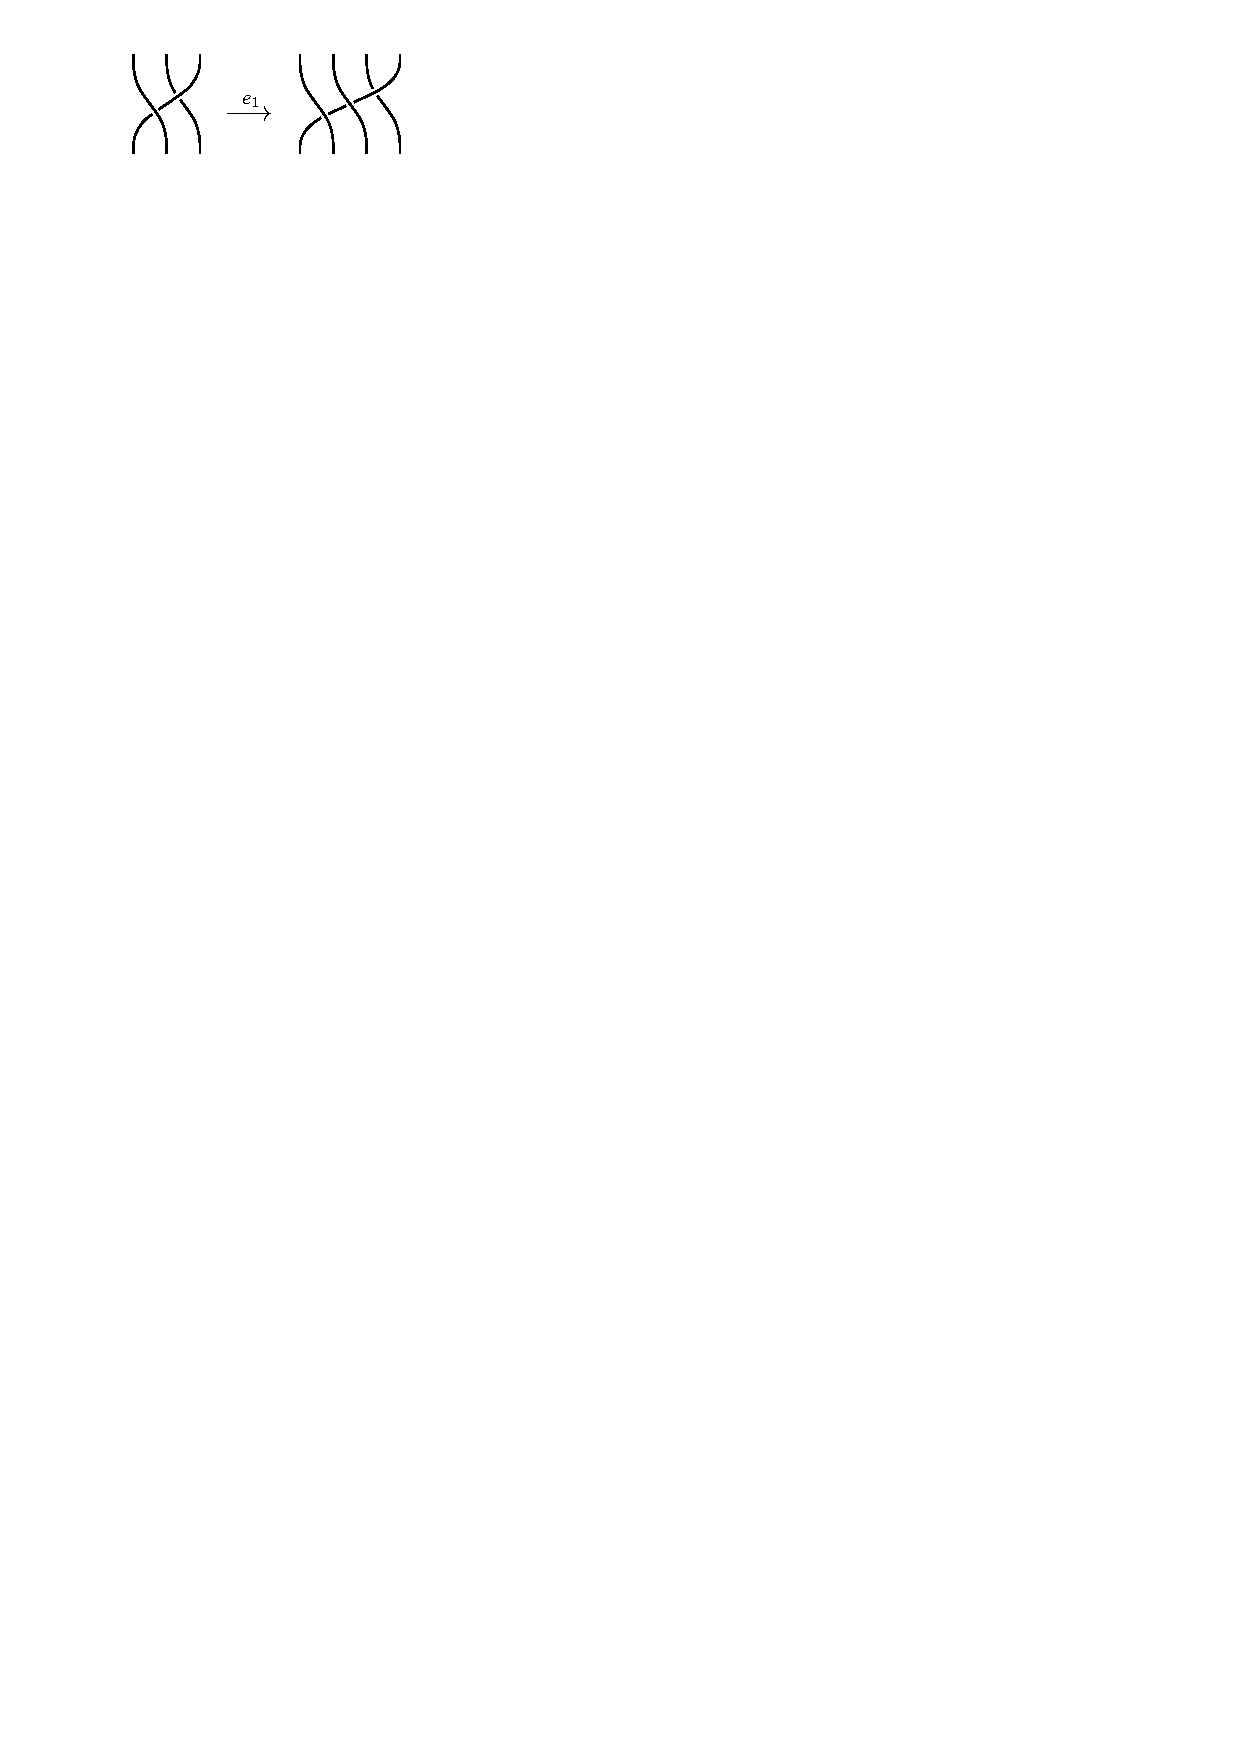
\includegraphics[width=60mm]{pictures/cabling.pdf}
\caption{Example of the cabling operation}
\label{cabling}}
\end{figure}


\begin{figure}[htbp]
\noindent\centering{
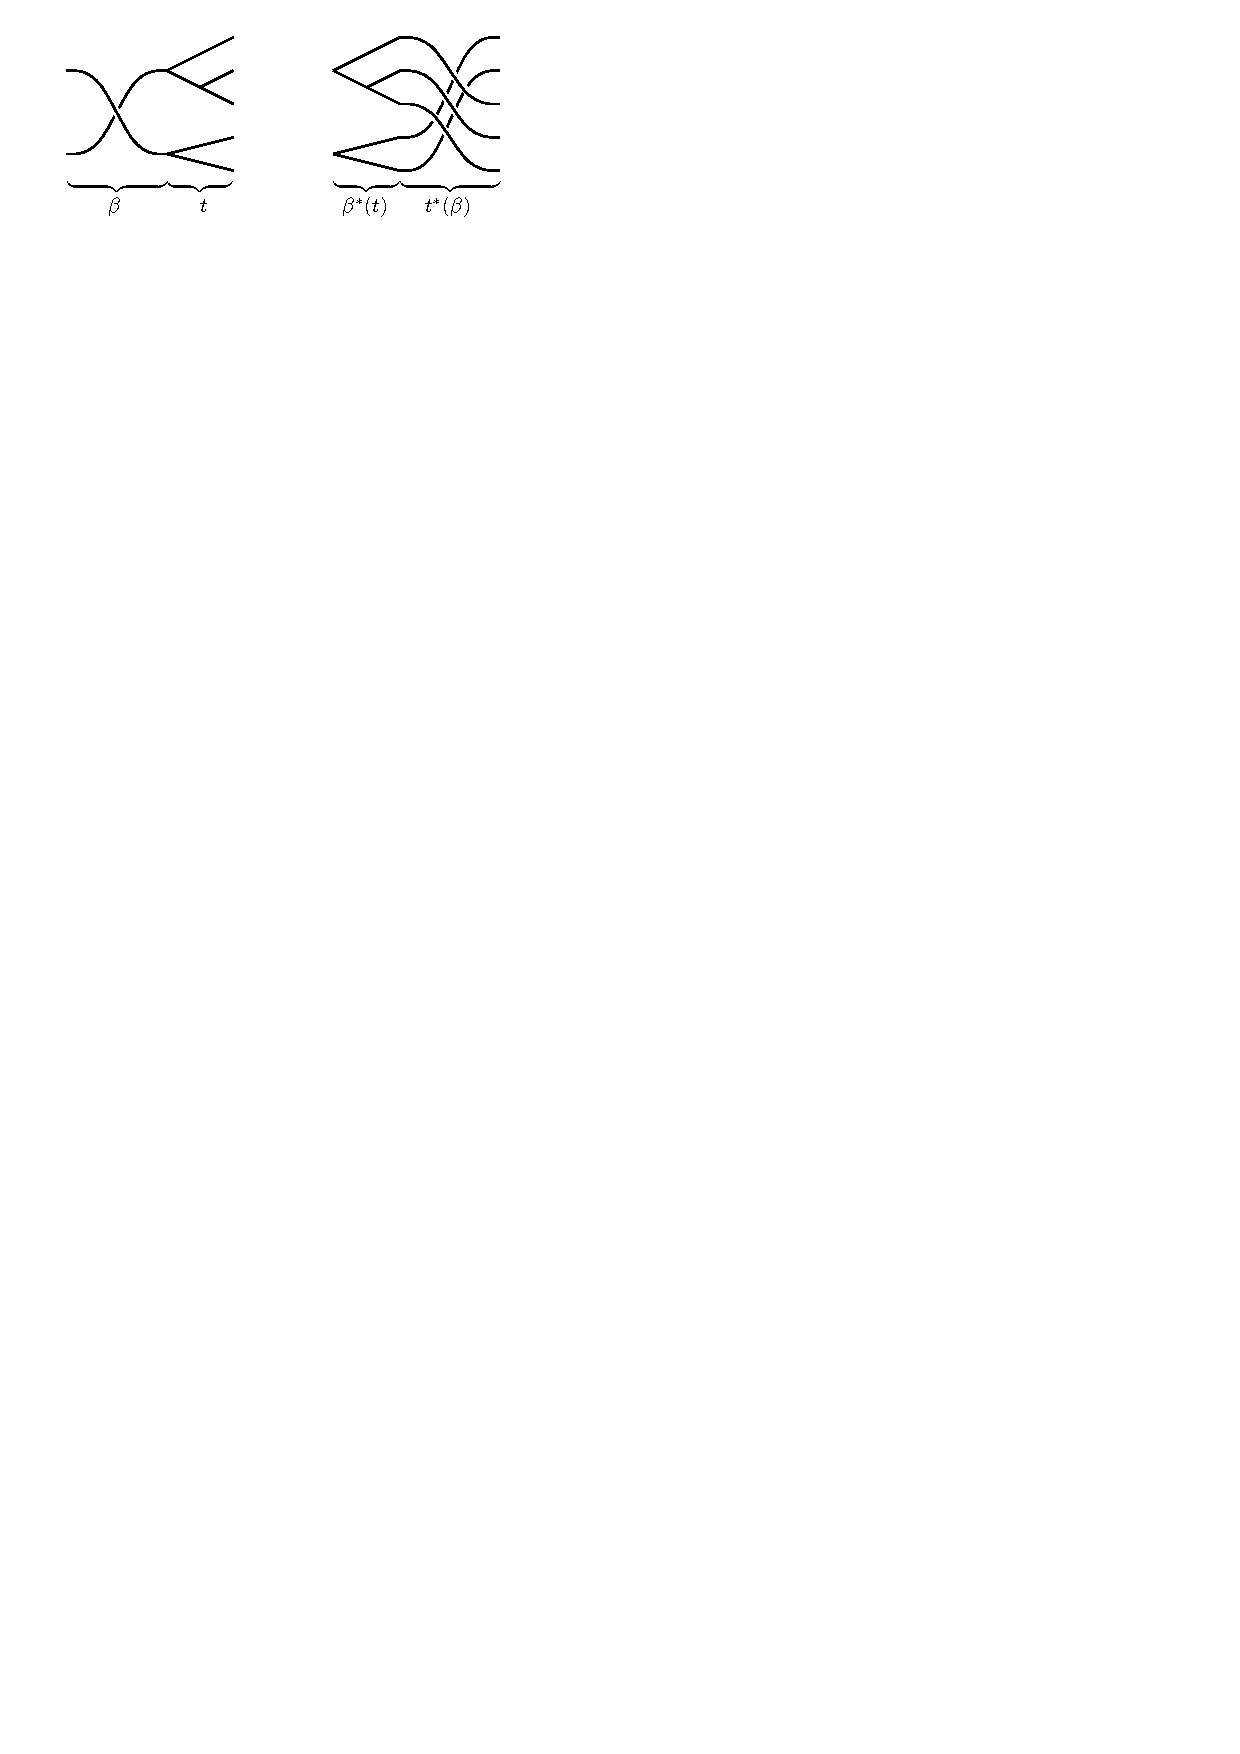
\includegraphics[width=100mm]{pictures/action_eg.pdf}
\caption{Example of a morphism $2 \to 5$ structure maps in $\Tau B$}
\label{actionOrigin}}
\end{figure}

\subsubsection{The hyperoctahedral crossed $\Tau$-group}
We now describe a specific crossed $\mathcal{T}$-group $H_*$. For each $n \geq 1$, define
\[
H_n = (\mathbb{Z}/2)^n \rtimes \Sigma_n,
\]
where the symmetric group $\Sigma_n$ acts on $(\mathbb{Z}/2)^n$ by permuting coordinates. This group is commonly called the \emph{hyperoctahedral group} or, in combinatorial contexts, the \emph{group of signed permutations}.

We define maps $e_i \colon H_n \longrightarrow H_{n+1}$ for $1 \leq i \leq n$ by:
\[
e_i((\varepsilon_1, \ldots, \varepsilon_n), \sigma) = ((\varepsilon_1, \ldots, \varepsilon_i, \varepsilon_i, \ldots, \varepsilon_n), e_i^{\varepsilon_i}(\sigma)),
\]
where:
\begin{itemize}
    \item $e_i^0(\sigma)$ denotes the standard cabling operation for permutations, analogous to the braid group cabling,
    \item $e_i^1(\sigma)$ denotes \emph{twisted cabling}, where the $i$-th strand is replaced by two intersecting strands, as illustrated in Figure~\ref{fig:cablingpic}.
\end{itemize}


\begin{remark}
Elements of $H_n$ can be visualized as $n$ strands with mod~2 twists, permuted according to $\sigma$. The maps $e_i$ then correspond to inserting either parallel or intersecting strands at position~$i$.

\begin{figure}[h]
  \centering
  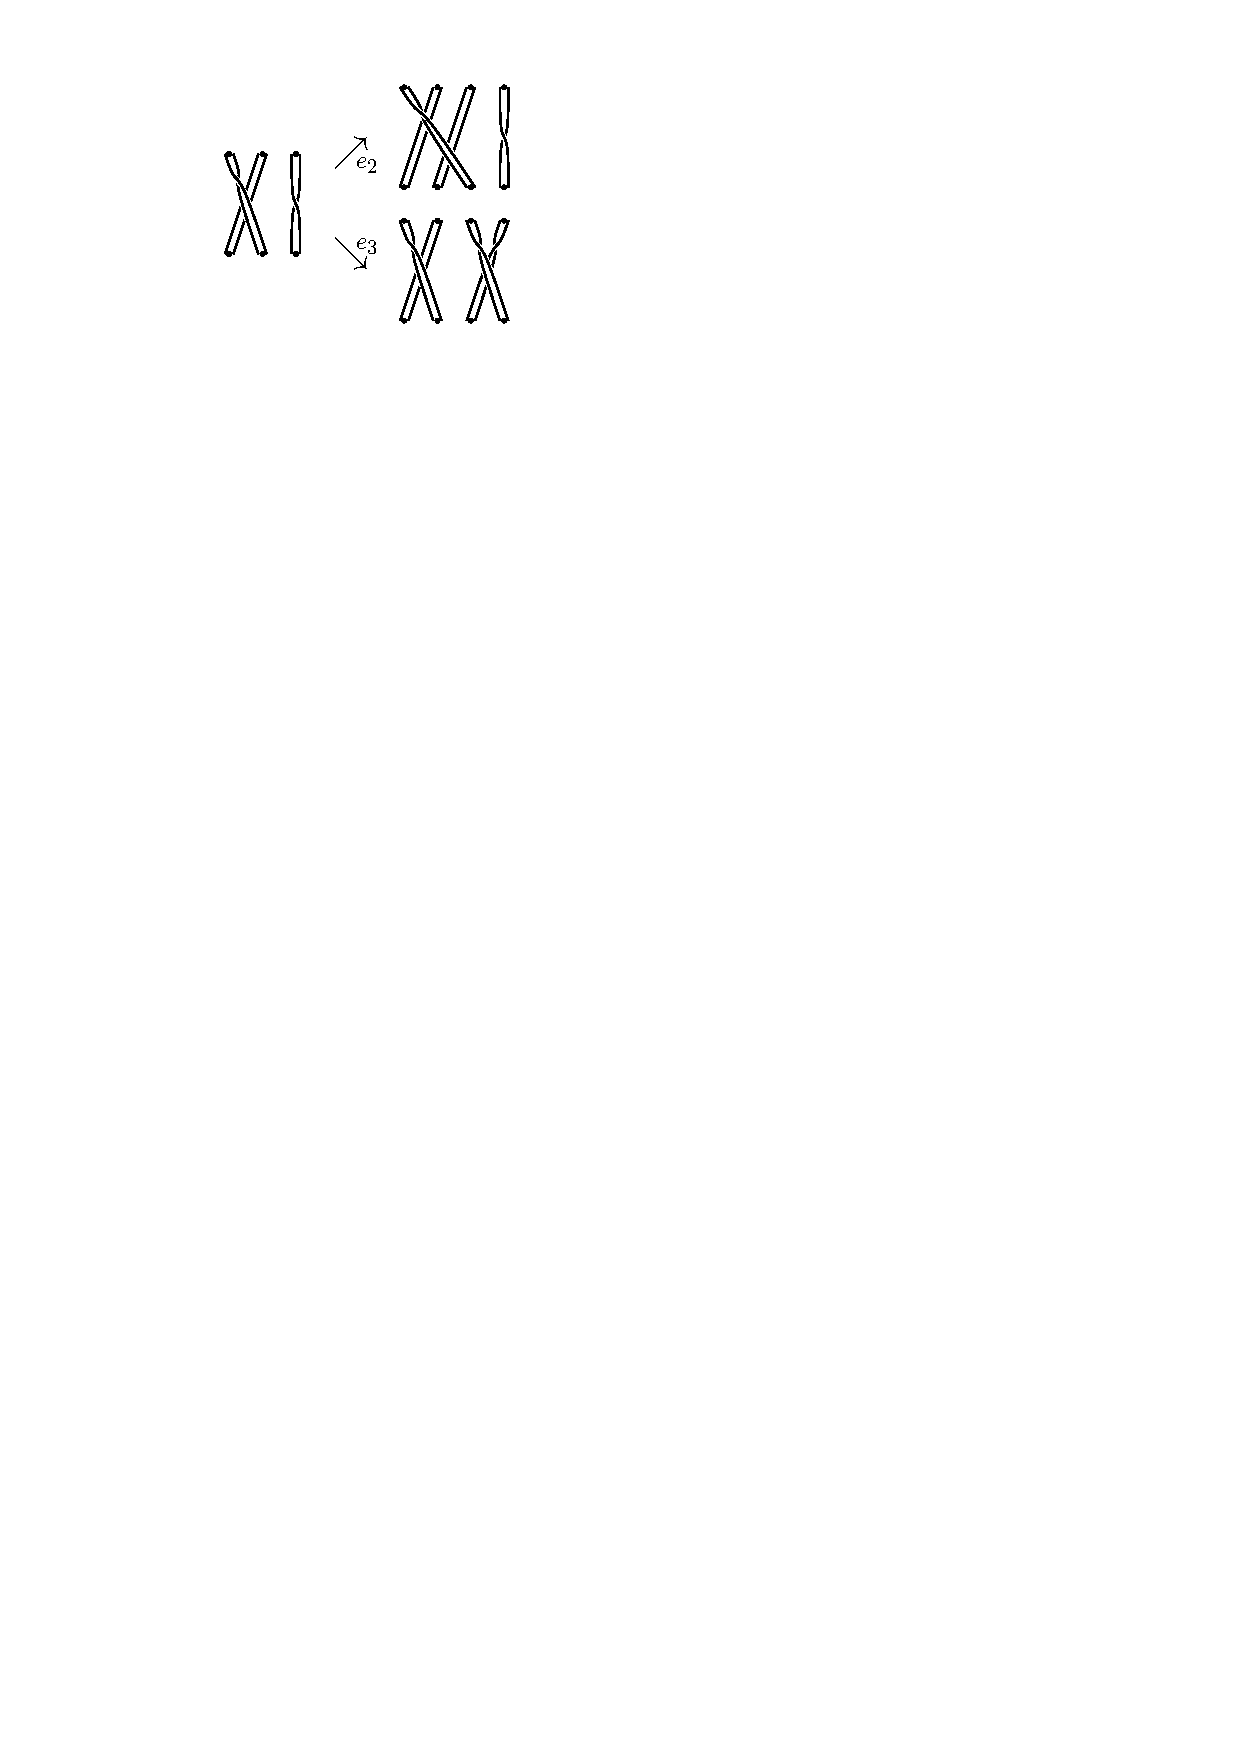
\includegraphics[width=0.3\textwidth]{pictures/zaplet-per.pdf}
  \caption{Multiplication by vertical concatenation and the action on \([n]\).}
  \label{fig:cablingpic}
\end{figure}
\end{remark}

\subsection{Connections with crossed simplicial groups}
Now that we have defined injective $\cc$-groups we can elaborate on the connections between crossed simplicial groups and crossed $\Tau$-groups, announced above. 

By definition, a crossed $\Delta$-group is a sequence of groups $G_0, G_1, G_2, \ldots$ together with morphisms $d_i : G_n \to G_{n-1}$ and $s_i : G_{n-1} \to G_n$ satisfying simplicial identities and crossed group properties. Note that identities in $\Tau$ between $e_i$'s are all present in $\Delta$ as simplicial identities ivolving $s_i$'s. Thus $\{G_i\}$'s  also form a crossed $\Tau$-group. Also, there is the simplicial identity $s_jd_j = \id$ which implies that $s_i$ are all injective functions. Thus we have proved the following lemma.


\begin{lemma}\label{Crossed-Tau}
    Any crossed simplicial group tautologically defines an injective crossed $\Tau$ group. 
\end{lemma}


\subsection{Connections with cloning systems}

Recall the definition of a cloning system due to M.~Zaremsky and S.~Witzel \cite{zaremsky2022usersguidecloningsystems}. 

\begin{definition}
A cloning system consists of a directed system of groups (a functor $i \colon \ZZ_{\ge 1} \to \Grp$, where $i([n]) =: G_n$) together with:
\begin{enumerate}
\item group homomorphisms $\rho_n \colon G_n \to \Sigma_n$ for each $n$, and
\item set maps $\kappa_k^n \colon G_n \to G_{n+1}$ for $1 \le k \le n$, called \emph{cloning functions}.
\end{enumerate}
These data are required to satisfy a list of axioms (see \cite{zaremsky2022usersguidecloningsystems}).
\end{definition}
Given a cloning system $(i, \{\rho_n\}_{n \ge 1}, \{\kappa_k^n\}_{n \ge 1, 1 \le k \le n})$, one associates a Thompson-like group whose elements are triples $[T_+, g, T_-]$, where $g \in G_n$ and $T_+$, $T_-$ are rooted binary trees with $n$ leaves (see \cite{zaremsky2022usersguidecloningsystems} for the precise construction). For each cloning system there is a corresponding $\Tau$-crossed group. The following observation is an immediate unpacking of the definitions.
\begin{lemma}\label{lemma:cloning_crossed}
Let $(i, \{\rho_n\}_{n \ge 1}, \{\kappa_k^n\}_{n \ge 1, 1 \le k \le n})$ be a cloning system. Then the assignment $n \mapsto G_n$ defines a crossed $\Tau$-group with $e_i$ given by $\kappa_i$.
\end{lemma}

It is worth noting that a system of structure maps $G_n \xrightarrow{i_{n,m}} G_m$ is not essential for defining a Thompson-like group. This was already observed by S.~Witzel in \cite{Witzel_2019}, where an alternative formulation based on the \emph{internal indirect product} of categories was introduced. The definition arising from crossed $\Tau$-groups is essentially equivalent to Witzel’s formulation. However, our approach makes the connection with algebraic topology more transparent and facilitates results such as Theorem~\ref{Theorem-B}.


\section{Structure theorem and its implications}
\begin{theorem}[Structure theorem, c.f.~\cite{fied_loday}]\label{thm:Categorical-structure-thm}
    Let $G$ be a $\Tau$-crossed group, then there exists a natural exact sequence of $\Tau$-crossed groups.
    $$1 \to \Tau P \to \Tau G \to \Tau H,$$
    where $H$ is the hyperoctahedral crossed $\Tau$-group and $P$ is an genuine $\Tau$-group. 
\end{theorem}
\begin{proof} This proof follows the proof of Theorem~3.6 of~\cite{fied_loday}.

    Consider the left action of $G_n$ on $\Tau(n, n + 1)$. Since $\Tau(n, n + 1)$ is an $n$-element set, this defines a group homomorphism $\pi_S \colon G_n \to 
    \Sigma_n$. 
    
    Note that by formulas from Definition~\ref{def_berger} in a crossed $\Tau$-group one has
     $$e_i^*(g_1g_2) = (g_2^*(e_i))^*(g_1)\cdot e_i^*(g_2) = e_{g_2^{-1}(i)}(g_1)e_i(g_2).$$
     It follows that $e_i$ acts homomorphically on the kernel of $\pi_S$. However, this kernel can be not closed under the $e_i$-th still. 

     We will restrict the subgroup $\ker \pi_S$ to a smaller one so that it becomes closed under $e_i$'s. 
    
     Define $\pi \colon G_n \to (\ZZ/2)^{\oplus n} \rtimes \Sigma_n $ as
     $$g \mapsto{\pi}((\varepsilon_1, \ldots, \varepsilon_n), \pi_S(g)), $$
     where $\varepsilon_i = 1$ if $e_i(g)$ acts on $\{i, i+1\}$ as a transposition and 0 otherwise. 
    
    Put $P_n := \ker \pi \trianglelefteq G_n$. We need to check that if $g \in P_n$, then $e_i(g) \in P_{n+1}$. It is straightforward that  $e_ie_j(g)$ acts trivially on $\{1, \ldots, n+2\}$. 
\end{proof}

Using the theorem \ref{thm:Categorical-structure-thm} one can derive an analogous classification result for generalized $\Tau$-Thompson's groups.
\begin{theorem}\label{thm:Group-structure}
    Let $\F_\Tau(G)$ be a generalized $\Tau$-Thompson's group, then there exists a natural short exact sequence of generalized $\Tau$-Thompson's groups: 
    $$1 \to \colim_{t \in \Tau_0} N_t \to \F_\Tau(G) \to \F_\Tau(H),$$
    where $N$ is a genuine $\Tau$-group.
\end{theorem}
Before we proceed with the proof we want to mention that for $G = \{B_n\}$ the theorem above specializes to a well known short exact sequence. Mainly, in this case the middle group is the braided Thompson's group $\F_\Tau(G) = bV$. Its projection to $\F_\Tau(H)$ has the Thompson's group $V$ as its image. Its kernel has been studied from different perspectives. For example, in~\cite{zaremsky2018normalsubgroupsbraidedthompson} it is called $P_{br}$.


\begin{proof}[Proof of Theorem~\ref{thm:Group-structure}]
    By writing $\F_\Tau (G)$ we implicitly assume that $G$ is an injective crossed $\Tau$-group. 
    Consider the exact sequence of crossed $\Tau$-groups given by \ref{thm:Categorical-structure-thm}: 
    $$1 \to \Tau N \to \Tau G \xrightarrow{\alpha} \Tau H.$$
    
    The kernel $K =\ker\{\F_\Tau(G) \to \F_\Tau(N)\}$ consists of triples $(t_1, g, t_2)$ such that $(t_1, \alpha(g), t_2) = 1$ in $\F_\Tau(N)$. Using Lemma~\ref{Normal-form} we obtain the following description: 

    \begin{equation}\label{rewrite-kernel}
      K =\ker\{\F_\Tau(G) \to \F_\Tau(N)\} = \{(t, g, t)\; | \; t \in \Tau_0, g\in G_{|t|}, \alpha(g)= 1\}. 
    \end{equation}
    The map $\colim_{t \in \Tau_0} H_t \to K$ is given by $H_t \ni g \mapsto (t, g, t)$. Using the description \ref{rewrite-kernel} it is easy to see that it is an isomorphism.
\end{proof}















































\appendix
\section{Routine verifications}

To work with localizations, we will need the following useful lemma, which is a classical result in the theory of Ore categories (see \cite{belk2007thompsonsgroupf}).

\begin{lemma}\label{word-problem-loc}
Let $\cc$ be an Ore category. Consider two formal fractions $p_1q_1^{-1}$ and $p_2q_2^{-1}$ in the localization. They are equal, i.e., $p_1q_1^{-1} = p_2q_2^{-1}$, if and only if there exist $r_1, r_2 \in \Arr(\cc)$ such that the following diagram commutes:
\[
\begin{tikzcd}
  && \bullet \\
  \\
  \bullet && \bullet && \bullet \\
  \\
  && \bullet
  \arrow["{p_1}"', from=1-3, to=3-1]
  \arrow["{p_2}", from=1-3, to=3-5]
  \arrow["{r_1}", from=3-1, to=3-3]
  \arrow["{r_2}"', from=3-5, to=3-3]
  \arrow["{q_1}", from=5-3, to=3-1]
  \arrow["{q_2}"', from=5-3, to=3-5]
\end{tikzcd}.
\]
\end{lemma}


\begin{proof}[Proof of Lemma~\ref{CrossedOreLocalize}]\ \\ 
    
    \textbf{Right Cancellability}. For $a, b, c \in \cc$ let $(\alpha, g), (\gamma, r) : b \to c$ and $(\beta, h) : \alpha \to \beta$ be morphisms such that
    $(\alpha, g)\cdot(\beta, h) = (\gamma, r)\cdot(\beta, h)$ or, unfolding the definition,
    $$(\alpha \circ g_* (\beta),\, \beta^*(g) \cdot h) = (\gamma \circ r_* (\beta),\, \beta^*(r) \cdot h).$$
    In the second coordinate by the injectiveness of $\beta^*$ we get $g = r$ and then by the cancellability in $\cc$ we get $\alpha = \gamma$. 

    \textbf{Left Cancellability}. Same argument, but one uses the fact that $g_*$ is a bijection. 

    \textbf{Common right multiples}. For two arrow $(\alpha, g), (\gamma, r) \in \Arr(\cc G_*)$, using existance of common right multiples property for $\cc$ we get two arrows $A, B \in \Arr(\cc)$ such that $\alpha A = \gamma B$. Put $\beta := (g^{-1})_*(A), \delta := (r^{-1})_*(B)$ and $h := (\beta^*(g))^{-1}, p := (\delta^*(r))^{-1}$. Thus two following products coincide by definition of $A, B$: 
    $$(\alpha, g)(\beta, h) = (\alpha \cdot g_*(\beta), \beta^*(g) \cdot h) = (\alpha A, 1),$$
    $$(\gamma, r) (\delta, p) = (\gamma \cdot r_*(\delta), \delta^*(r) \cdot p) = (\gamma B, 1).$$

Putting $G = \{1\}$ we get that the condition (2) is necessary. 
\end{proof}


\begin{proof}[Proof of Lemma~\ref{Normal-form}]
    By Lemma~\ref{word-problem-loc} there exist $r_1, r_2 \in \cc G$ so that $t_1g r_1 = r_2 = t_2r_1$. By the definition of $\cc G$ decompose $r_1 = T_1 h_1, r_2 = T_2h_2$ with $T_i \in \Arr(\cc), h_i \in G_\ast$, thus
    $$t_1 g T_1h_1 = T_2h_2 = t_2T_1h_1.$$
    It follows that $T_1^*(g) = 1$, by the injectivity we get that $g = 1$, $h_1 = h_2$. We deduce from above the equality $t_1T_1h_1 = t_2T_1 h_1$. Canceling from right we get that $t_1 = t_2$.
\end{proof}








%%%%%%%%%%%%%%%%%%%%%%%%%%%%%%%%%%%%%%%%%%
%%%%%%%%%% Subgroup theorem %%%%%%%%%%%%%%
%%%%%%%%%%%%%%%%%%%%%%%%%%%%%%%%%%%%%%%%%%


\begin{proof}[Proof of Lemma~\ref{Lm:OrePullBack}]
    Pullback of left (right) cancellable categories is left (right) cancellable. Thus, we need to prove that $\ee \times_\bb \cc$ has common right multiples.
    Suppose that morphisms $f = (e_1, c_1)$ and $q = (e_2, c_2)$ have the same domain. Then by axiom O2, there exist morphisms $r, s$ such that $c_1r = c_2s$ in $\cc$. 
    Let $P_o$ be the bijection induced by $p$ on the sets of objects of $\dom\; e_1 / \ee \to \dom \;c_1 / \bb$. Put $\varphi := c_1 r$ to be the composition in $\cc$. 

% https://q.uiver.app/#q=WzAsOCxbMCwzLCJjXzEiXSxbMiwzLCJjXzMiXSxbMSwyLCJjXzIiXSxbMywyLCJjXzQiXSxbMCwxLCJlXzEiXSxbMSwwLCJlXzIiXSxbMiwxLCJlXzMiXSxbMywwLCJlXzQiXSxbMCwyLCJwXzEiXSxbMCwxLCJxXzEiLDJdLFsyLDMsIlxcZXhpc3RcXDsgcl8xIiwwLHsibGFiZWxfcG9zaXRpb24iOjMwLCJzdHlsZSI6eyJib2R5Ijp7Im5hbWUiOiJkYXNoZWQifX19XSxbMSwzLCJcXGV4aXN0IFxcOyBzXzEiLDIseyJzdHlsZSI6eyJib2R5Ijp7Im5hbWUiOiJkYXNoZWQifX19XSxbNCwwLCIiLDIseyJzdHlsZSI6eyJ0YWlsIjp7Im5hbWUiOiJtYXBzIHRvIn0sImJvZHkiOnsibmFtZSI6ImRvdHRlZCJ9fX1dLFs1LDIsIiIsMix7InN0eWxlIjp7InRhaWwiOnsibmFtZSI6Im1hcHMgdG8ifSwiYm9keSI6eyJuYW1lIjoiZG90dGVkIn19fV0sWzYsMSwiIiwyLHsic3R5bGUiOnsidGFpbCI6eyJuYW1lIjoibWFwcyB0byJ9LCJib2R5Ijp7Im5hbWUiOiJkb3R0ZWQifX19XSxbNywzLCIiLDIseyJzdHlsZSI6eyJ0YWlsIjp7Im5hbWUiOiJtYXBzIHRvIn0sImJvZHkiOnsibmFtZSI6ImRvdHRlZCJ9fX1dLFs0LDUsInBfMiIsMV0sWzQsNiwicV8yIiwxLHsibGFiZWxfcG9zaXRpb24iOjcwfV0sWzUsNywicl8yIiwyLHsic3R5bGUiOnsiYm9keSI6eyJuYW1lIjoiZGFzaGVkIn19fV0sWzYsNywic18yIiwyLHsic3R5bGUiOnsiYm9keSI6eyJuYW1lIjoiZGFzaGVkIn19fV1d
\[\begin{tikzcd}
	& {*} && {*} \\
	{*} && {*} \\
	& {*} && {*} \\
	{*} && {*}
	\arrow["{r_2}"', dashed, from=1-2, to=1-4]
	\arrow[dotted, maps to, from=1-2, to=3-2]
	\arrow[dotted, maps to, from=1-4, to=3-4]
	\arrow["{e_1}"{description}, from=2-1, to=1-2]
	\arrow["{e_2}"{description, pos=0.7}, from=2-1, to=2-3]
	\arrow[dotted, maps to, from=2-1, to=4-1]
	\arrow["{s_2}"', dashed, from=2-3, to=1-4]
	\arrow[dotted, maps to, from=2-3, to=4-3]
	\arrow["{\exists\; r}"{pos=0.3}, dashed, from=3-2, to=3-4]
	\arrow["{c_1}", from=4-1, to=3-2]
	\arrow["{c_2}"', from=4-1, to=4-3]
	\arrow["{\exists \; s}"', dashed, from=4-3, to=3-4]
\end{tikzcd}\]

Set $r_2 := e_1^{-1}P_o^{-1}(\varphi)$ and $s_2 := e_2^{-1}P_o^{-1}(\varphi)$. Then $(r_2, r)$ is a correctly defined morphism in $\ee \times_\bb \cc$ since 
$p(r_2) = p(e_1^{-1}) \cdot \varphi = c_1^{-1}c_1r = r$ belongs to $\cc$. By the same reasoning $(s_2, s)$ is a correctly defined morphism in $\ee \times_\bb \cc$.
By definition $e_1 r_2 = e_2 s_2$, thus the morphisms $(r_2, r)$ and $(s_2, s)$ provide common right multiples.
\end{proof}


\begin{proof}[Proof of Lemma~\ref{technical1}]
    Let us denote $\qq := \cc \times_{\Loc \cc} E$. By Lemma~\ref{Lm:OrePullBack} the category $\qq$ is an Ore category, thus $\Loc \qq$ is its groupoid of fractions.

    First, we prove \textbf{essential surjectivity} of the functor $\Loc \qq \to \ee$. Note that the set of objects of $\qq$ is the same as the set of objects of $\Loc \qq$. Take an object $e \in \ee$. Then $(e, p(e)) \in \qq$ is the preimage of $e$. 

    Next, we prove that the functor $\Loc \qq \to \ee$ \textbf{ is full}. For this we prove that any morphism in $\ee$ can be represented as a fraction of two morphisms in $\qq$.
     Take a morphism $f \colon a \to b \in \ee$. Since $\Loc \cc$ is the groupoid of fractions of $\cc$, $p(f)$ can be factored as $\varphi_1 \varphi_2^{-1}$ for some $\varphi_1, \varphi_2 \in \cc$. 
    % https://q.uiver.app/#q=WzAsNSxbMCwwLCJhIl0sWzIsMCwiYiJdLFswLDIsInAoYSkiXSxbMiwyLCJwKGIpIl0sWzEsMywiXFxidWxsZXQiXSxbMCwxLCJmIl0sWzIsMywicChmKSJdLFsyLDQsIlxcdmFycGhpXzEiLDJdLFszLDQsIlxcdmFycGhpXzIiXV0=
\[\begin{tikzcd}
	{p(a)} && {p(b)} \\
	& \bullet
	\arrow["{p(f)}", from=1-1, to=1-3]
	\arrow["{\varphi_1}"', from=1-1, to=2-2]
	\arrow["{\varphi_2}", from=1-3, to=2-2]
\end{tikzcd}\]

Let $P_o$ be the bijection induced by $p$ on the sets of objects of $a / \ee \to p(a) / \Loc \cc$.

Define $f_1 = P_o^{-1}(\varphi_1), f_2 := f^{-1}f_1$. Then $(f_1, p(f_1))$ and $(f_2, p(f_2))$ are correctly defined morphisms in $\qq$ and $f_1f_2^{-1} = f$. Thus the functor is full. 

Lastly, we need to prove that the functor $\Loc \qq \to \ee$ \textbf{is faithful}. Since we work with groupoids we need to check that if image of some $f$ is $\id_e$ then $f$ itself is $\id_e$ for some $e$. 
Take $f = (g_\cc, g_\ee)(h_\cc, h_\ee)^{-1}$ in $\Loc \qq$ such that its image in $\ee$ is $\id$. It is easy to see that the image is $g_\ee h_\ee^{-1}$. We need to prove that it implies that $g_\cc = h_\cc$. We use Lemma \ref{word-problem-loc}. 
Since $g_\cc h_\cc^{-1} = p(g_\ee h_\ee^{-1}) = \id$ we have a commutative diagram in $\cc$ of the form
% https://q.uiver.app/#q=WzAsNSxbMCwyLCJcXGJ1bGxldCJdLFs0LDIsIlxcYnVsbGV0Il0sWzIsNCwiXFxidWxsZXQiXSxbMiwwLCJcXGJ1bGxldCJdLFsyLDIsIlxcYnVsbGV0Il0sWzAsMywiZ19cXG1hdGhjYWx7Q30iXSxbMSwzLCJoX1xcbWF0aGNhbHtDfSIsMl0sWzAsMiwiXFx0ZXh0c2Z7aWR9IiwyXSxbMSwyLCJcXHRleHRzZntpZH0iXSxbMyw0LCJyXzEiXSxbMiw0LCJyXzIiLDJdXQ==
\[\begin{tikzcd}
	&& \bullet \\
	\\
	\bullet && \bullet && \bullet \\
	\\
	&& \bullet
	\arrow["{r_1}", from=1-3, to=3-3]
	\arrow["{g_\mathcal{C}}", from=3-1, to=1-3]
	\arrow["{\textsf{id}}"', from=3-1, to=5-3]
	\arrow["{h_\mathcal{C}}"', from=3-5, to=1-3]
	\arrow["{\textsf{id}}", from=3-5, to=5-3]
	\arrow["{r_2}"', from=5-3, to=3-3]
\end{tikzcd}\]
That is, $g_\cc r_1 = r_2$ and $h_\cc r_1 = r_2$ which imply by cancellability that $g_\cc = h_\cc$

\end{proof}


\begin{proof}[Proof of Lemma~\ref{technical2}]
    First, note that the category $\qq$ can also be presented as the pullback $\cc \to \Loc(\cc \; G) \leftarrow \ee$. This follows from a well-known categorical result (also known as the pasting lemma), that in a commutative diagram as below, where the right square is a pullback, the left square is a pullback if and only if the outer rectangle is a pullback.
    \[\begin{tikzcd}
	\bullet & \bullet & \bullet \\
	\bullet & \bullet & \bullet
	\arrow[from=1-1, to=1-2]
	\arrow[from=1-1, to=2-1]
	\arrow[from=1-2, to=1-3]
	\arrow[from=1-2, to=2-2]
	\arrow["\lrcorner"{anchor=center, pos=0.125}, draw=none, from=1-2, to=2-3]
	\arrow[from=1-3, to=2-3]
	\arrow[from=2-1, to=2-2]
	\arrow[from=2-2, to=2-3]
\end{tikzcd}\]


Let us denote by $p \colon \ee \to \Loc \; \cc G$ the covering map on the right.
If $(f_\cc, f_\ee)$ is an isomorphism with inverse $(g_\cc, g_\ee)$ then $f = g = \id_e$ since $\cc$ is gaunt. Then, $f_\ee$ is also an $\id$ morphism by the covering properties. Thus, $\qq$ is gaunt.

Now we prove that each morphism in $X$ factors uniquely as a morphism in $\qq$ followed by an isomorphism. Take $(f_{\cc G}, f_\ee)$ a morphim in $X$. 
To prove the existence of such decomposition, represent $f_{\cc G} = f_\cc f_G$, consider $P_o$ to be the bijection induced by $p$ on the sets of objects 
of $\dom \; f_\ee / \ee \to \dom \; f_\cc / \Loc \cc$ and take $f_\ee^1 = P_o^{-1}(f_\cc)$ and $f_\ee^2 = (f_\ee^1)^{-1}f_\ee$. Then obviously $(f_\cc, f_\ee^1)(f_G, f_\ee^2)$ is the desired decomposition.
To prove the uniqueness suppose that $(f_1, e_1)(f_2, e_2) = (g_1, t_1)(g_2, t_2)$ for some $(f_1, e_1), (g_1, t_1) \in \qq$ and $(f_2, e_2), (g_2, t_2)$ isomorphisms.
Then by uniqueness of decomposition in $\cc G$ we have $f_1 = g_1, f_2 = g_2$. By covering properties, there is a unique morphism $\psi \in \ee$ with $\dom\; \psi = \dom \; e_1$ such that $p(\psi) = f_1$. 
Thus, $e_1 = t_1 = \psi$, thus the decomposition is unique.

% To prove that $X$ is the category of a crossed group over $\qq$ we prove that any morphism in $X$ can be uniquely factored as a composition of a morphism from $\qq$ and an automorphism.
% To prove the existence of factoring, take a morphism in $X$, it is given by a pair $(f_{\cc G}, f_\ee)$ where $f_{\cc G} \in \cc G$ and $f_\ee \in \ee$. 
% By definition, there exists a unique decomposition $f_{\cc G} = f_\cc \cdot f_G$ for some $f_\cc \in \cc$ and $f_G \in G_{\cod \; f_\cc}$. 
% Let $P_o$ be the bijection induced by $p$ on the sets of objects of $\dom \; f_\ee / \ee \to \dom \; f_\cc / \Loc \cc$. 
% Let $\varphi_\cc := P_o^{-1}(f_\cc)$ be a morphism in $\ee$ and put $\varphi_G := $

% % https://q.uiver.app/#q=WzAsNixbMCwwLCJlXzEiXSxbMiwwLCJlXzIiXSxbNCwwLCJlXzIiXSxbMCwyLCJjXzEiXSxbMiwyLCJjXzIiXSxbNCwyLCJjXzIiXSxbMyw0LCJcXGluIFxcbWF0aGNhbHtDfSIsMl0sWzQsNSwiXFxpbiBHX3tjXzJ9IiwyXSxbMCwzLCIiLDIseyJzdHlsZSI6eyJ0YWlsIjp7Im5hbWUiOiJtYXBzIHRvIn0sImJvZHkiOnsibmFtZSI6ImRvdHRlZCJ9fX1dLFsxLDQsIiIsMix7InN0eWxlIjp7InRhaWwiOnsibmFtZSI6Im1hcHMgdG8ifSwiYm9keSI6eyJuYW1lIjoiZG90dGVkIn19fV0sWzIsNSwiIiwwLHsic3R5bGUiOnsidGFpbCI6eyJuYW1lIjoibWFwcyB0byJ9LCJib2R5Ijp7Im5hbWUiOiJkb3R0ZWQifX19XSxbMCwxLCJcXGV4aXN0cyIsMSx7InN0eWxlIjp7ImJvZHkiOnsibmFtZSI6ImRhc2hlZCJ9fX1dLFswLDIsIlxcZXhpc3RzIiwwLHsibGFiZWxfcG9zaXRpb24iOjQwLCJjdXJ2ZSI6LTMsInN0eWxlIjp7ImJvZHkiOnsibmFtZSI6ImRhc2hlZCJ9fX1dXQ==
% \[\begin{tikzcd}
% 	{e_1} && {e_2} && {e_2} \\
% 	\\
% 	{c_1} && {c_2} && {c_2}
% 	\arrow["\exists"{description}, dashed, from=1-1, to=1-3]
% 	\arrow["\exists"{pos=0.4}, curve={height=-18pt}, dashed, from=1-1, to=1-5]
% 	\arrow[dotted, maps to, from=1-1, to=3-1]
% 	\arrow[dotted, maps to, from=1-3, to=3-3]
% 	\arrow[dotted, maps to, from=1-5, to=3-5]
% 	\arrow["{\in \mathcal{C}}"', from=3-1, to=3-3]
% 	\arrow["{\in G_{c_2}}"', from=3-3, to=3-5]
% \end{tikzcd}\]

% A morphism $(c_1, e_1) \to (c_2, e_2)$ in the category $X$ is a pair of morphisms $f \colon c_1 \to c_2$ and $g \colon e_1 \to e_2$. The first of them uniquely decomposes as a composition $f = f_\cc f_{G_{c_2}}$, and we consider the liftings of these morphisms under the covering in the slice category $e_1/E$, which gives the desired factorization. It is unique due to the uniqueness of the decomposition of $f$.
\end{proof}

\begin{lemma}
    Let $\cc$ be a category with wide subcategory $\ww \subseteq \cc$ such that each morphism in $\cc$ can be uniquely decomposed as a morphism in $\ww$ followed by an isomorphism. Then, $\cc$ is equivalent to $\ww G$ for some crossed $\ww$ group $G$.
\end{lemma}
\begin{proof}
    We prove that the skeleton of $\cc$ is a category of a crossed $\ww$ group. It is trivial that $\ww$ is gaunt. Take a set of representatives $\{g_i\}_{i \in \ii}$ for each isomorphism class. 
    Denote as $[g_i]$ the set of objects of $\cc$ that are isomorphic to $g_i$. For each $h \in [g_i]$ choose an isomorphism $\alpha^h_i : h \to g_i$. 
    This defines a functor $\cc \to \bb$ to the full subcategory spanned by $g_i$'s. 
    
\end{proof}

% \printbibliography


% % \bibliography{references}
% % \bibliographystyle{alphaurl}



\end{document}
